% ════════════════════════════════════════════
% 模型求解（5.3.4）
% ════════════════════════════════════════════
\subsubsection{结果与解读}

基于上述框架，本节依次估计全模型与最终模型，并完成诊断与验证。求解环境为 Python 3，使用 NumPy 与 SciPy 实现最小二乘与 HC3 协方差，使用 statsmodels 完成 Huber 稳健回归与 Gamma 广义线性模型的对照估计，随机种子固定为 20261122。

首先给出全模型 M1 的系数表。由表\ref{tab:q3_full}可知，M1 的样本内拟合优度为 0.2069、调整拟合优度为 0.1633、整体 F 值为 4.7465，整体显著性成立。帖子类型的参照类为 Photo，Status 的系数为 1.152、Video 为 1.588，均在 1\% 水平显著；Link 为 0.122、p 值 0.643，与 Photo 无显著差异。内容主题 2 与主题 3 的系数分别为 $-0.477$ 与 $-0.313$，均显著为负。付费系数为 0.337、p 值 0.005，方向与前述敏感性对照一致。最值得注意的是粉丝规模：系数 0.836 看似为正，但 HC3 标准误高达 3.819，p 值 0.827，95\% 置信区间为 $-6.669$ 至 8.341，区间宽度超过系数本身一个数量级，说明该参数没有被数据识别。

\begin{longtable}{>{\centering\arraybackslash}p{0.17\textwidth}>{\centering\arraybackslash}p{0.085\textwidth}>{\centering\arraybackslash}p{0.085\textwidth}>{\centering\arraybackslash}p{0.07\textwidth}>{\centering\arraybackslash}p{0.07\textwidth}>{\centering\arraybackslash}p{0.08\textwidth}>{\centering\arraybackslash}p{0.08\textwidth}>{\centering\arraybackslash}p{0.08\textwidth}}
  \caption{全模型 M1 系数表}
  \label{tab:q3_full} \\
  \toprule
  变量 & 系数 & HC3\newline 标准误 & t 值 & p 值 & CI 下限 & CI 上限 & VIF \\
  \midrule
  \endfirsthead
  \caption{全模型 M1 系数表（续）} \\
  \toprule
  变量 & 系数 & HC3\newline 标准误 & t 值 & p 值 & CI 下限 & CI 上限 & VIF \\
  \midrule
  \endhead
  \bottomrule
  \endfoot
  常数项 & $-0.249$ & 43.361 & $-0.006$ & 0.995 & $-85.453$ & 84.956 & — \\
  $\log X_1$ & 0.836 & 3.819 & 0.219 & 0.827 & $-6.669$ & 8.341 & 124.905 \\
  类型 Status & 1.152 & 0.124 & 9.262 & $<$0.001 & 0.908 & 1.396 & 1.277 \\
  类型 Link & 0.122 & 0.262 & 0.466 & 0.642 & $-0.393$ & 0.638 & 1.136 \\
  类型 Video & 1.588 & 0.401 & 3.956 & $<$0.001 & 0.799 & 2.377 & 1.063 \\
  主题 2 & $-0.477$ & 0.136 & $-3.516$ & $<$0.001 & $-0.743$ & $-0.210$ & 1.787 \\
  主题 3 & $-0.313$ & 0.134 & $-2.344$ & 0.020 & $-0.576$ & $-0.051$ & 1.531 \\
  月份 2 & 0.814 & 0.418 & 1.945 & 0.052 & $-0.008$ & 1.636 & 3.735 \\
  月份 3 & $-0.174$ & 0.622 & $-0.280$ & 0.780 & $-1.397$ & 1.049 & 12.749 \\
  月份 4 & 0.170 & 0.986 & 0.172 & 0.863 & $-1.768$ & 2.108 & 37.686 \\
  月份 5 & $-0.077$ & 1.235 & $-0.063$ & 0.950 & $-2.505$ & 2.350 & 45.158 \\
  月份 6 & $-0.168$ & 1.465 & $-0.114$ & 0.909 & $-3.047$ & 2.712 & 79.837 \\
  月份 7 & $-0.034$ & 1.609 & $-0.021$ & 0.983 & $-3.196$ & 3.127 & 100.837 \\
  月份 8 & $-0.254$ & 1.698 & $-0.150$ & 0.881 & $-3.592$ & 3.083 & 76.254 \\
  月份 9 & $-0.509$ & 1.774 & $-0.287$ & 0.774 & $-3.996$ & 2.978 & 87.661 \\
  月份 10 & $-0.861$ & 1.811 & $-0.476$ & 0.635 & $-4.420$ & 2.697 & 142.994 \\
  月份 11 & $-0.363$ & 1.841 & $-0.197$ & 0.844 & $-3.980$ & 3.255 & 115.705 \\
  月份 12 & $-0.506$ & 1.871 & $-0.271$ & 0.787 & $-4.184$ & 3.171 & 131.298 \\
  星期 2 & 0.093 & 0.198 & 0.470 & 0.639 & $-0.296$ & 0.482 & 1.760 \\
  星期 3 & $-0.021$ & 0.193 & $-0.107$ & 0.915 & $-0.399$ & 0.358 & 1.771 \\
  星期 4 & 0.259 & 0.210 & 1.234 & 0.218 & $-0.154$ & 0.672 & 1.848 \\
  星期 5 & $-0.092$ & 0.178 & $-0.515$ & 0.607 & $-0.441$ & 0.258 & 1.797 \\
  星期 6 & $-0.160$ & 0.186 & $-0.864$ & 0.388 & $-0.525$ & 0.204 & 1.933 \\
  星期 7 & $-0.221$ & 0.176 & $-1.255$ & 0.210 & $-0.566$ & 0.125 & 1.898 \\
  时段 凌晨 & 0.166 & 0.114 & 1.460 & 0.145 & $-0.057$ & 0.389 & 1.322 \\
  时段 下午晚间 & 0.073 & 0.162 & 0.447 & 0.655 & $-0.246$ & 0.391 & 1.530 \\
  付费 & 0.337 & 0.120 & 2.808 & 0.005 & 0.101 & 0.573 & 1.077 \\
\end{longtable}

表\ref{tab:q3_collin}把共线证据集中列出。M1 的最大 VIF 为 142.99，出现在 10 月；粉丝规模的 VIF 为 124.91；标准化条件数为 48.52，超过 30 的严重阈值。月份哑变量的 VIF 自 3 月起快速上升，到 10 月达到峰值，与粉丝规模的 VIF 互为镜像，说明二者在争抢同一段变异。增量 F 检验显示，在已含月份固定效应的模型中加入粉丝规模，F 值仅 0.0495、p 值 0.824，几乎不增加任何解释力。M2 剔除粉丝规模后，最大 VIF 降至 3.232、条件数降至 6.356，共线问题基本消除。GVIF 方面，粉丝规模的 $\mathrm{GVIF}^{1/2}$ 为 11.176，远超阈值 2.24，其余变量组均低于 1.28。

\begin{longtable}{>{\centering\arraybackslash}p{0.29\textwidth}>{\centering\arraybackslash}p{0.25\textwidth}>{\centering\arraybackslash}p{0.12\textwidth}>{\centering\arraybackslash}p{0.23\textwidth}}
  \caption{共线性诊断}
  \label{tab:q3_collin} \\
  \toprule
  诊断项 & 对象 & 数值 & 判断 \\
  \midrule
  \endfirsthead
  \caption{共线性诊断（续）} \\
  \toprule
  诊断项 & 对象 & 数值 & 判断 \\
  \midrule
  \endhead
  \bottomrule
  \endfoot
  M1 最大 VIF & 全部解释变量 & 142.994 & 超过 10，严重共线 \\
  M1 VIF & $\log X_1$ & 124.905 & 超过 10，严重共线 \\
  M1 VIF & 月份哑变量最大值 & 142.994 & 与 $\log X_1$ 互为镜像 \\
  M1 标准化条件数 & 全部解释变量 & 48.519 & 超过 30，数值不稳定 \\
  M1 增量 F 统计量 & 在 M2 基础上加入 $\log X_1$ & 0.0495 & 增量贡献极小 \\
  增量 F 检验 p 值 & 同上 & 0.824 & 不显著，系数不可识别 \\
  $R^2(\log X_1\sim\text{月份})$ & 月间趋势 & 0.9917 & 粉丝规模几乎由月份决定 \\
  月内方差占比 & 组内变异 & 0.0083 & 低于 0.05，月内信息不足 \\
  M2 最大 VIF & 全部解释变量 & 3.232 & 低于 5，可接受 \\
  M2 标准化条件数 & 全部解释变量 & 6.356 & 低于 30，通过 \\
  GVIF$^{1/2}$：$\log X_1$ & 自由度 1 & 11.176 & 超过阈值 2.24 \\
  GVIF$^{1/2}$：类型 & 自由度 3 & 1.073 & 未超过阈值 \\
  GVIF$^{1/2}$：主题 & 自由度 2 & 1.161 & 未超过阈值 \\
  GVIF$^{1/2}$：月份 & 自由度 11 & 1.278 & 未超过阈值 \\
  GVIF$^{1/2}$：星期 & 自由度 6 & 1.018 & 未超过阈值 \\
  GVIF$^{1/2}$：时段 & 自由度 2 & 1.083 & 未超过阈值 \\
  GVIF$^{1/2}$：付费 & 自由度 1 & 1.038 & 未超过阈值 \\
\end{longtable}

图\ref{fig:q3_vif}直观展示了共线处理前后的差异。左图中粉丝规模与 6 月至 12 月的月份哑变量全部越过 10 的参考线，最高接近 143；右图中最终模型的全部变量都落在 5 以下，最高的月份变量仅为 3.23。这说明剔除粉丝规模并非损失信息，而是把重复计数的时间维度合并为一个，使剩余系数可以稳定估计。

\begin{figure}[ht]
  \centering
  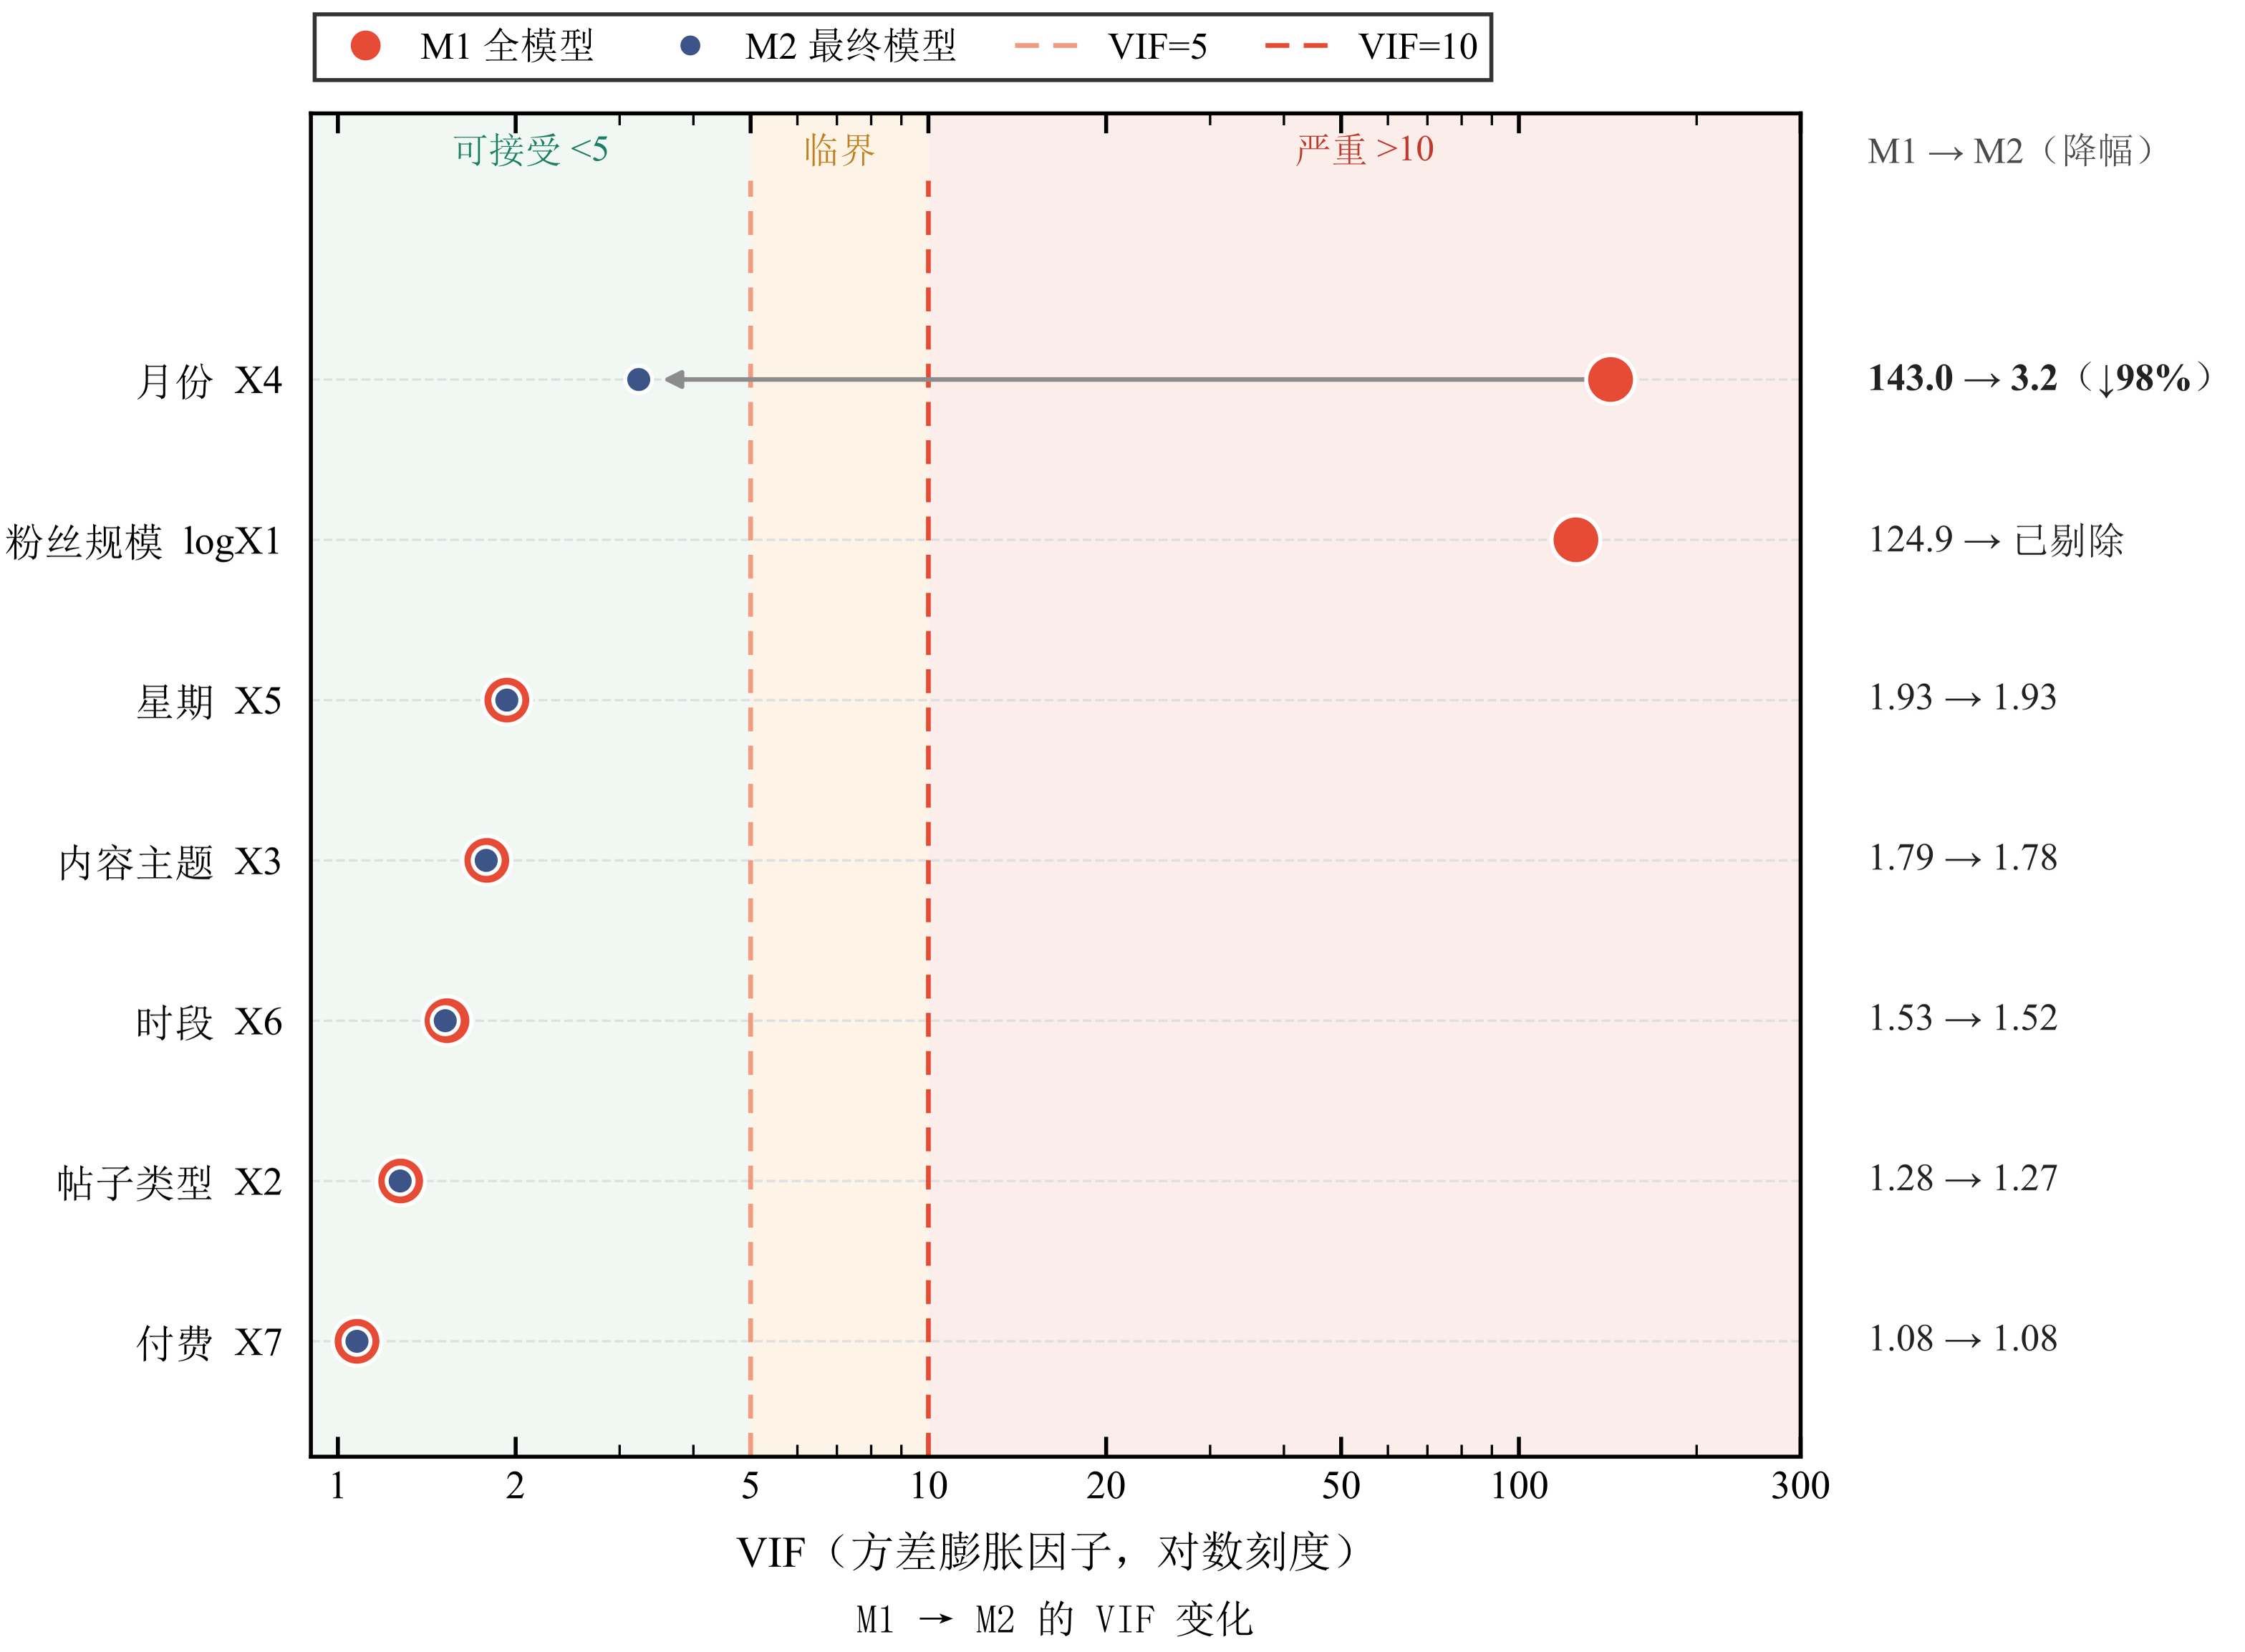
\includegraphics[width=0.72\textwidth]{../求解/问题三/结果/图7_共线性诊断.png}
  \caption{全模型与最终模型的方差膨胀因子}
  \label{fig:q3_vif}
\end{figure}

据此确定最终模型 M2，其主效应系数如表\ref{tab:q3_final}所示。常数项 9.247 对应参照组合（Photo、主题 1、1 月、周一、上午、自然）的基线对数曝光。Status 的系数为 1.154、p 值小于 0.001，折算为 $e^{1.154}=3.17$ 倍；Video 为 1.590、p 值小于 0.001，折算为 4.90 倍；Link 为 0.122、p 值 0.643，折算为 1.13 倍且不显著。主题 2 与主题 3 分别为 $-0.478$ 与 $-0.315$，折算为 0.62 倍与 0.73 倍。付费系数为 0.337、p 值 0.005，折算为 1.40 倍。月份与星期的系数为控制变量，正文不再逐一展开；全模型 M1 的完整估计见表\ref{tab:q3_full}，最终模型 M2 仅剔除粉丝规模一项。

\begin{longtable}{>{\centering\arraybackslash}p{0.17\textwidth}>{\centering\arraybackslash}p{0.085\textwidth}>{\centering\arraybackslash}p{0.085\textwidth}>{\centering\arraybackslash}p{0.07\textwidth}>{\centering\arraybackslash}p{0.07\textwidth}>{\centering\arraybackslash}p{0.08\textwidth}>{\centering\arraybackslash}p{0.08\textwidth}>{\centering\arraybackslash}p{0.08\textwidth}}
  \caption{最终模型 M2 主效应系数表}
  \label{tab:q3_final} \\
  \toprule
  变量 & 系数 & HC3\newline 标准误 & t 值 & p 值 & CI 下限 & CI 上限 & VIF \\
  \midrule
  \endfirsthead
  \caption{最终模型 M2 主效应系数表（续）} \\
  \toprule
  变量 & 系数 & HC3\newline 标准误 & t 值 & p 值 & CI 下限 & CI 上限 & VIF \\
  \midrule
  \endhead
  \bottomrule
  \endfoot
  常数项 & 9.247 & 0.205 & 45.062 & $<$0.001 & 8.844 & 9.650 & — \\
  类型 Status & 1.154 & 0.124 & 9.339 & $<$0.001 & 0.911 & 1.397 & 1.275 \\
  类型 Link & 0.122 & 0.262 & 0.464 & 0.643 & $-0.393$ & 0.636 & 1.136 \\
  类型 Video & 1.590 & 0.402 & 3.958 & $<$0.001 & 0.800 & 2.379 & 1.063 \\
  主题 2 & $-0.478$ & 0.135 & $-3.540$ & $<$0.001 & $-0.744$ & $-0.213$ & 1.783 \\
  主题 3 & $-0.315$ & 0.134 & $-2.353$ & 0.019 & $-0.578$ & $-0.052$ & 1.527 \\
  付费 & 0.337 & 0.120 & 2.823 & 0.005 & 0.103 & 0.572 & 1.077 \\
\end{longtable}

表\ref{tab:q3_compare}比较五种设定的拟合与预测表现。M1 与 M2 的样本内 $R^2$ 几乎相同（0.2069 与 0.2068），但 M2 少一个参数、调整 $R^2$ 略高（0.1650 对 0.1633），说明粉丝规模没有带来额外解释力。M3 与 M4 的 $R^2$ 分别为 0.1606 与 0.1664，低于 M2，表明月份固定效应比线性粉丝规模更能吸收时间变异。交叉验证的结果差距更大：M2 的 CV $R^2$ 为 0.1010，高于 M1 的 0.0972、M3 的 0.0935 与 M4 的 0.0972；M0 的 CV $R^2$ 为 $-0.0212$，说明不含任何变量的均值基线在样本外还不如直接用测试集均值。M2 的 CV RMSE 为 1.1007、CV MAE 为 0.8328，均为五者最小。

\begin{longtable}{>{\centering\arraybackslash}p{0.205\textwidth}>{\centering\arraybackslash}p{0.075\textwidth}>{\centering\arraybackslash}p{0.075\textwidth}>{\centering\arraybackslash}p{0.085\textwidth}>{\centering\arraybackslash}p{0.09\textwidth}>{\centering\arraybackslash}p{0.08\textwidth}>{\centering\arraybackslash}p{0.09\textwidth}>{\centering\arraybackslash}p{0.085\textwidth}}
  \caption{模型比较与十折交叉验证}
  \label{tab:q3_compare} \\
  \toprule
  模型 & 参数数 & $R^2$ & 调整 $R^2$ & 残差\newline 标准误 & CV $R^2$ & CV RMSE & CV MAE \\
  \midrule
  \endfirsthead
  \caption{模型比较与十折交叉验证（续）} \\
  \toprule
  模型 & 参数数 & $R^2$ & 调整 $R^2$ & 残差\newline 标准误 & CV $R^2$ & CV RMSE & CV MAE \\
  \midrule
  \endhead
  \bottomrule
  \endfoot
  M0 均值基线 & 1 & 0.0000 & 0.0000 & 1.1781 & $-0.0212$ & 1.1753 & 0.9133 \\
  M1 全模型 & 27 & 0.2069 & 0.1633 & 1.0776 & 0.0972 & 1.1031 & 0.8351 \\
  M2 月份固定效应 & 26 & 0.2068 & 0.1650 & 1.0765 & 0.1010 & 1.1007 & 0.8328 \\
  M3 仅 $\log X_1$ & 16 & 0.1606 & 0.1346 & 1.0959 & 0.0935 & 1.1065 & 0.8220 \\
  M4 $\log X_1$ 加线性月份 & 17 & 0.1664 & 0.1388 & 1.0933 & 0.0972 & 1.1042 & 0.8215 \\
\end{longtable}

图\ref{fig:q3_forest}以森林图形式展示最终模型的主效应。点估计按正负与显著性着色，横轴为 log1p 尺度，右侧标注折算后的倍数。Status 与 Video 的区间完全位于 0 的右侧，主题 2 与主题 3 的区间完全位于 0 的左侧，付费的区间也整体为正；Link 的区间跨越 0，对应 p 值 0.643。Video 的区间最宽，上界接近 2.38，这是仅 7 条视频帖带来的必然结果，解读时应强调方向而非精确倍数。

\begin{figure}[ht]
  \centering
  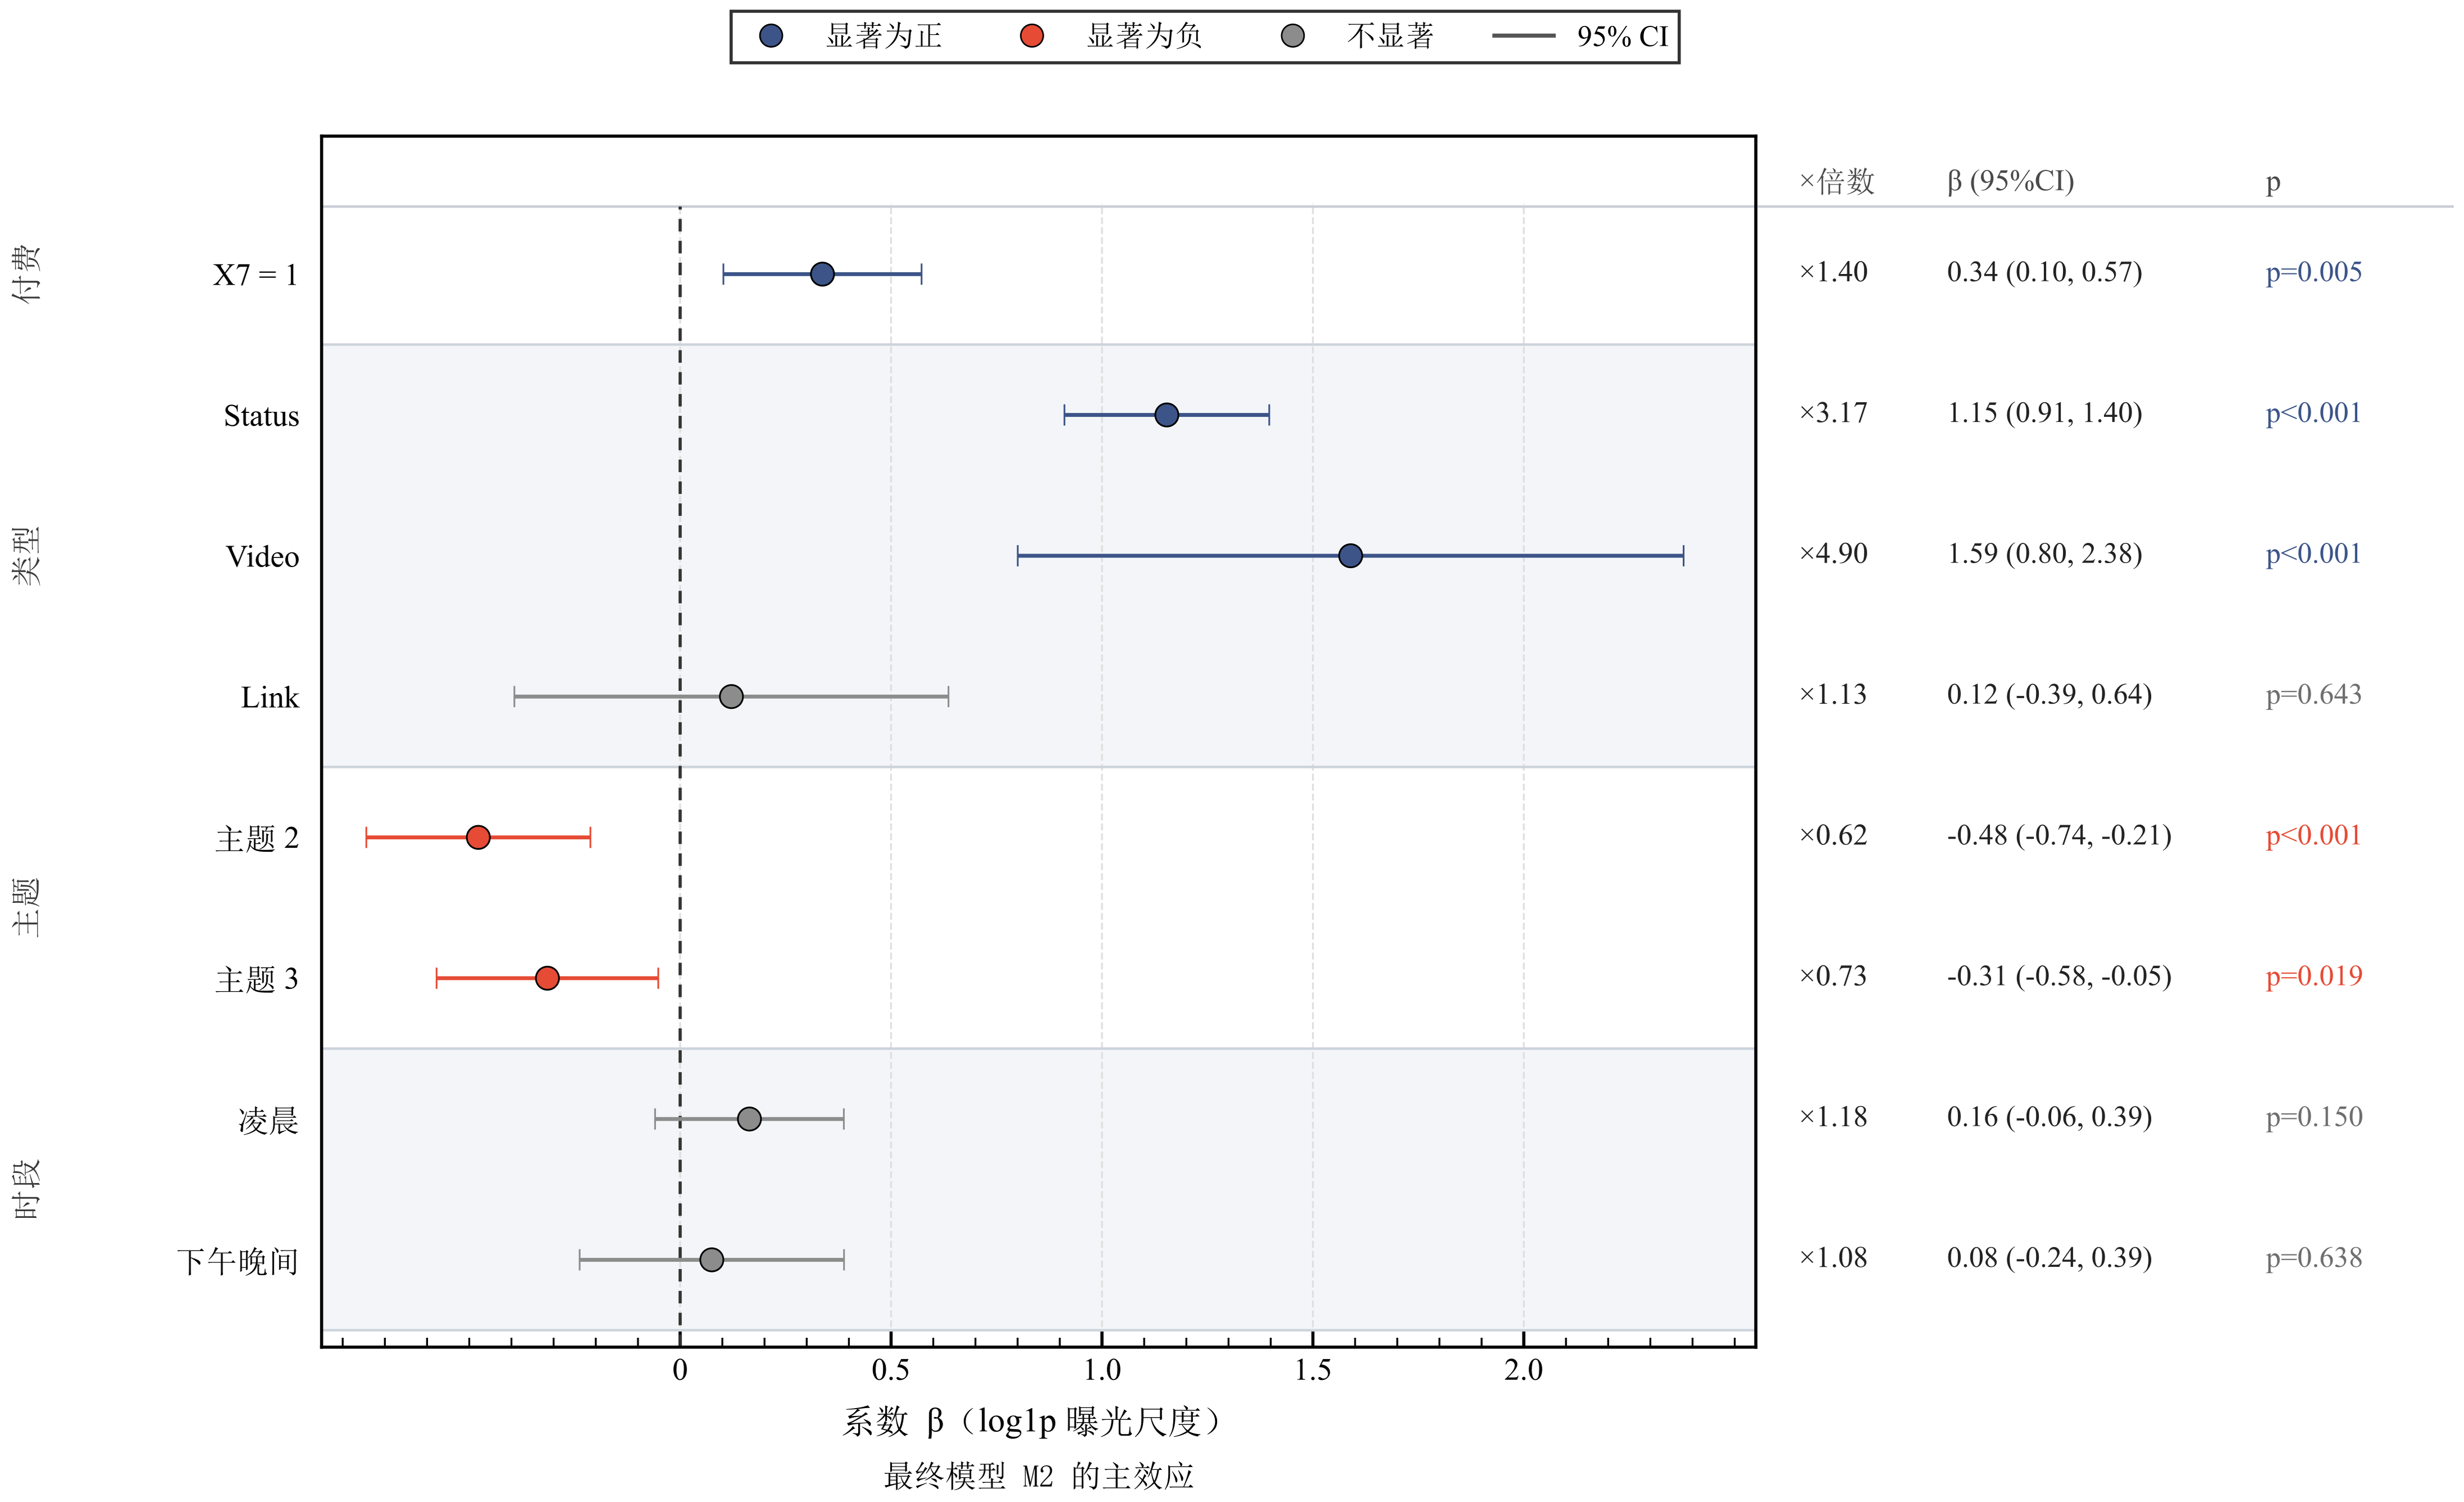
\includegraphics[width=0.64\textwidth]{../求解/问题三/结果/图6_最终模型系数森林图.png}
  \caption{最终模型主效应系数与 95\% 置信区间}
  \label{fig:q3_forest}
\end{figure}

表\ref{tab:q3_resid}报告残差诊断。Jarque--Bera 统计量为 120.36、p 值小于 0.001，残差仍偏离正态；Breusch--Pagan 统计量为 54.74、p 值 0.0005，存在异方差；White 检验统计量 266.52、p 值 0.030，同样拒绝同方差。这两项正是采用 HC3 标准误的理由。Ramsey RESET 的 F 值为 2.845、p 值 0.059，在 5\% 水平未检出函数形式误设；Durbin--Watson 为 2.052，接近 2；Cook 距离最大值为 0.0377，远小于 1，说明没有单条帖子主导估计；杠杆值超过 $2p/n=0.104$ 的观测有 10 个，属于高杠杆但未构成强影响。

\begin{longtable}{>{\centering\arraybackslash}p{0.12\textwidth}>{\centering\arraybackslash}p{0.30\textwidth}>{\centering\arraybackslash}p{0.11\textwidth}>{\centering\arraybackslash}p{0.09\textwidth}>{\centering\arraybackslash}p{0.22\textwidth}}
  \caption{残差诊断检验}
  \label{tab:q3_resid} \\
  \toprule
  模型 & 检验 & 统计量 & p 值 & 判断 \\
  \midrule
  \endfirsthead
  \caption{残差诊断检验（续）} \\
  \toprule
  模型 & 检验 & 统计量 & p 值 & 判断 \\
  \midrule
  \endhead
  \bottomrule
  \endfoot
  M1 & Jarque--Bera 正态性 & 118.973 & $<$0.001 & 残差非正态 \\
  M1 & Breusch--Pagan 异方差 & 56.518 & 0.0005 & 存在异方差 \\
  M1 & White 异方差 & 283.283 & 0.079 & 未检出 \\
  M1 & Ramsey RESET & 2.867 & 0.058 & 未检出设定误差 \\
  M1 & Durbin--Watson & 2.051 & — & 接近 2 \\
  M1 & Cook 距离最大值 & 0.049 & — & 无强影响点 \\
  M2 & Jarque--Bera 正态性 & 120.360 & $<$0.001 & 残差非正态 \\
  M2 & Breusch--Pagan 异方差 & 54.737 & 0.0005 & 存在异方差 \\
  M2 & White 异方差 & 266.519 & 0.030 & 存在异方差 \\
  M2 & Ramsey RESET & 2.845 & 0.059 & 未检出设定误差 \\
  M2 & Durbin--Watson & 2.052 & — & 接近 2 \\
  M2 & 高杠杆点个数 & 10 & — & 阈值 0.104 \\
  M2 & Cook 距离最大值 & 0.038 & — & 无强影响点 \\
\end{longtable}

图\ref{fig:q3_resid}把残差结构可视化。残差对拟合值呈水平带状分布，均值接近 0，但在低拟合值区略厚；Q--Q 图两端偏离参考线，对应少数极端曝光帖；尺度—位置图的平滑线基本水平，说明异方差主要来自尾部而非系统性趋势；标准化残差直方图峰值略高于正态曲线，尾部更厚。整体看，残差没有呈现明显的非线性或漏斗形，HC3 标准误足以应对剩余的异方差。

\begin{figure}[ht]
  \centering
  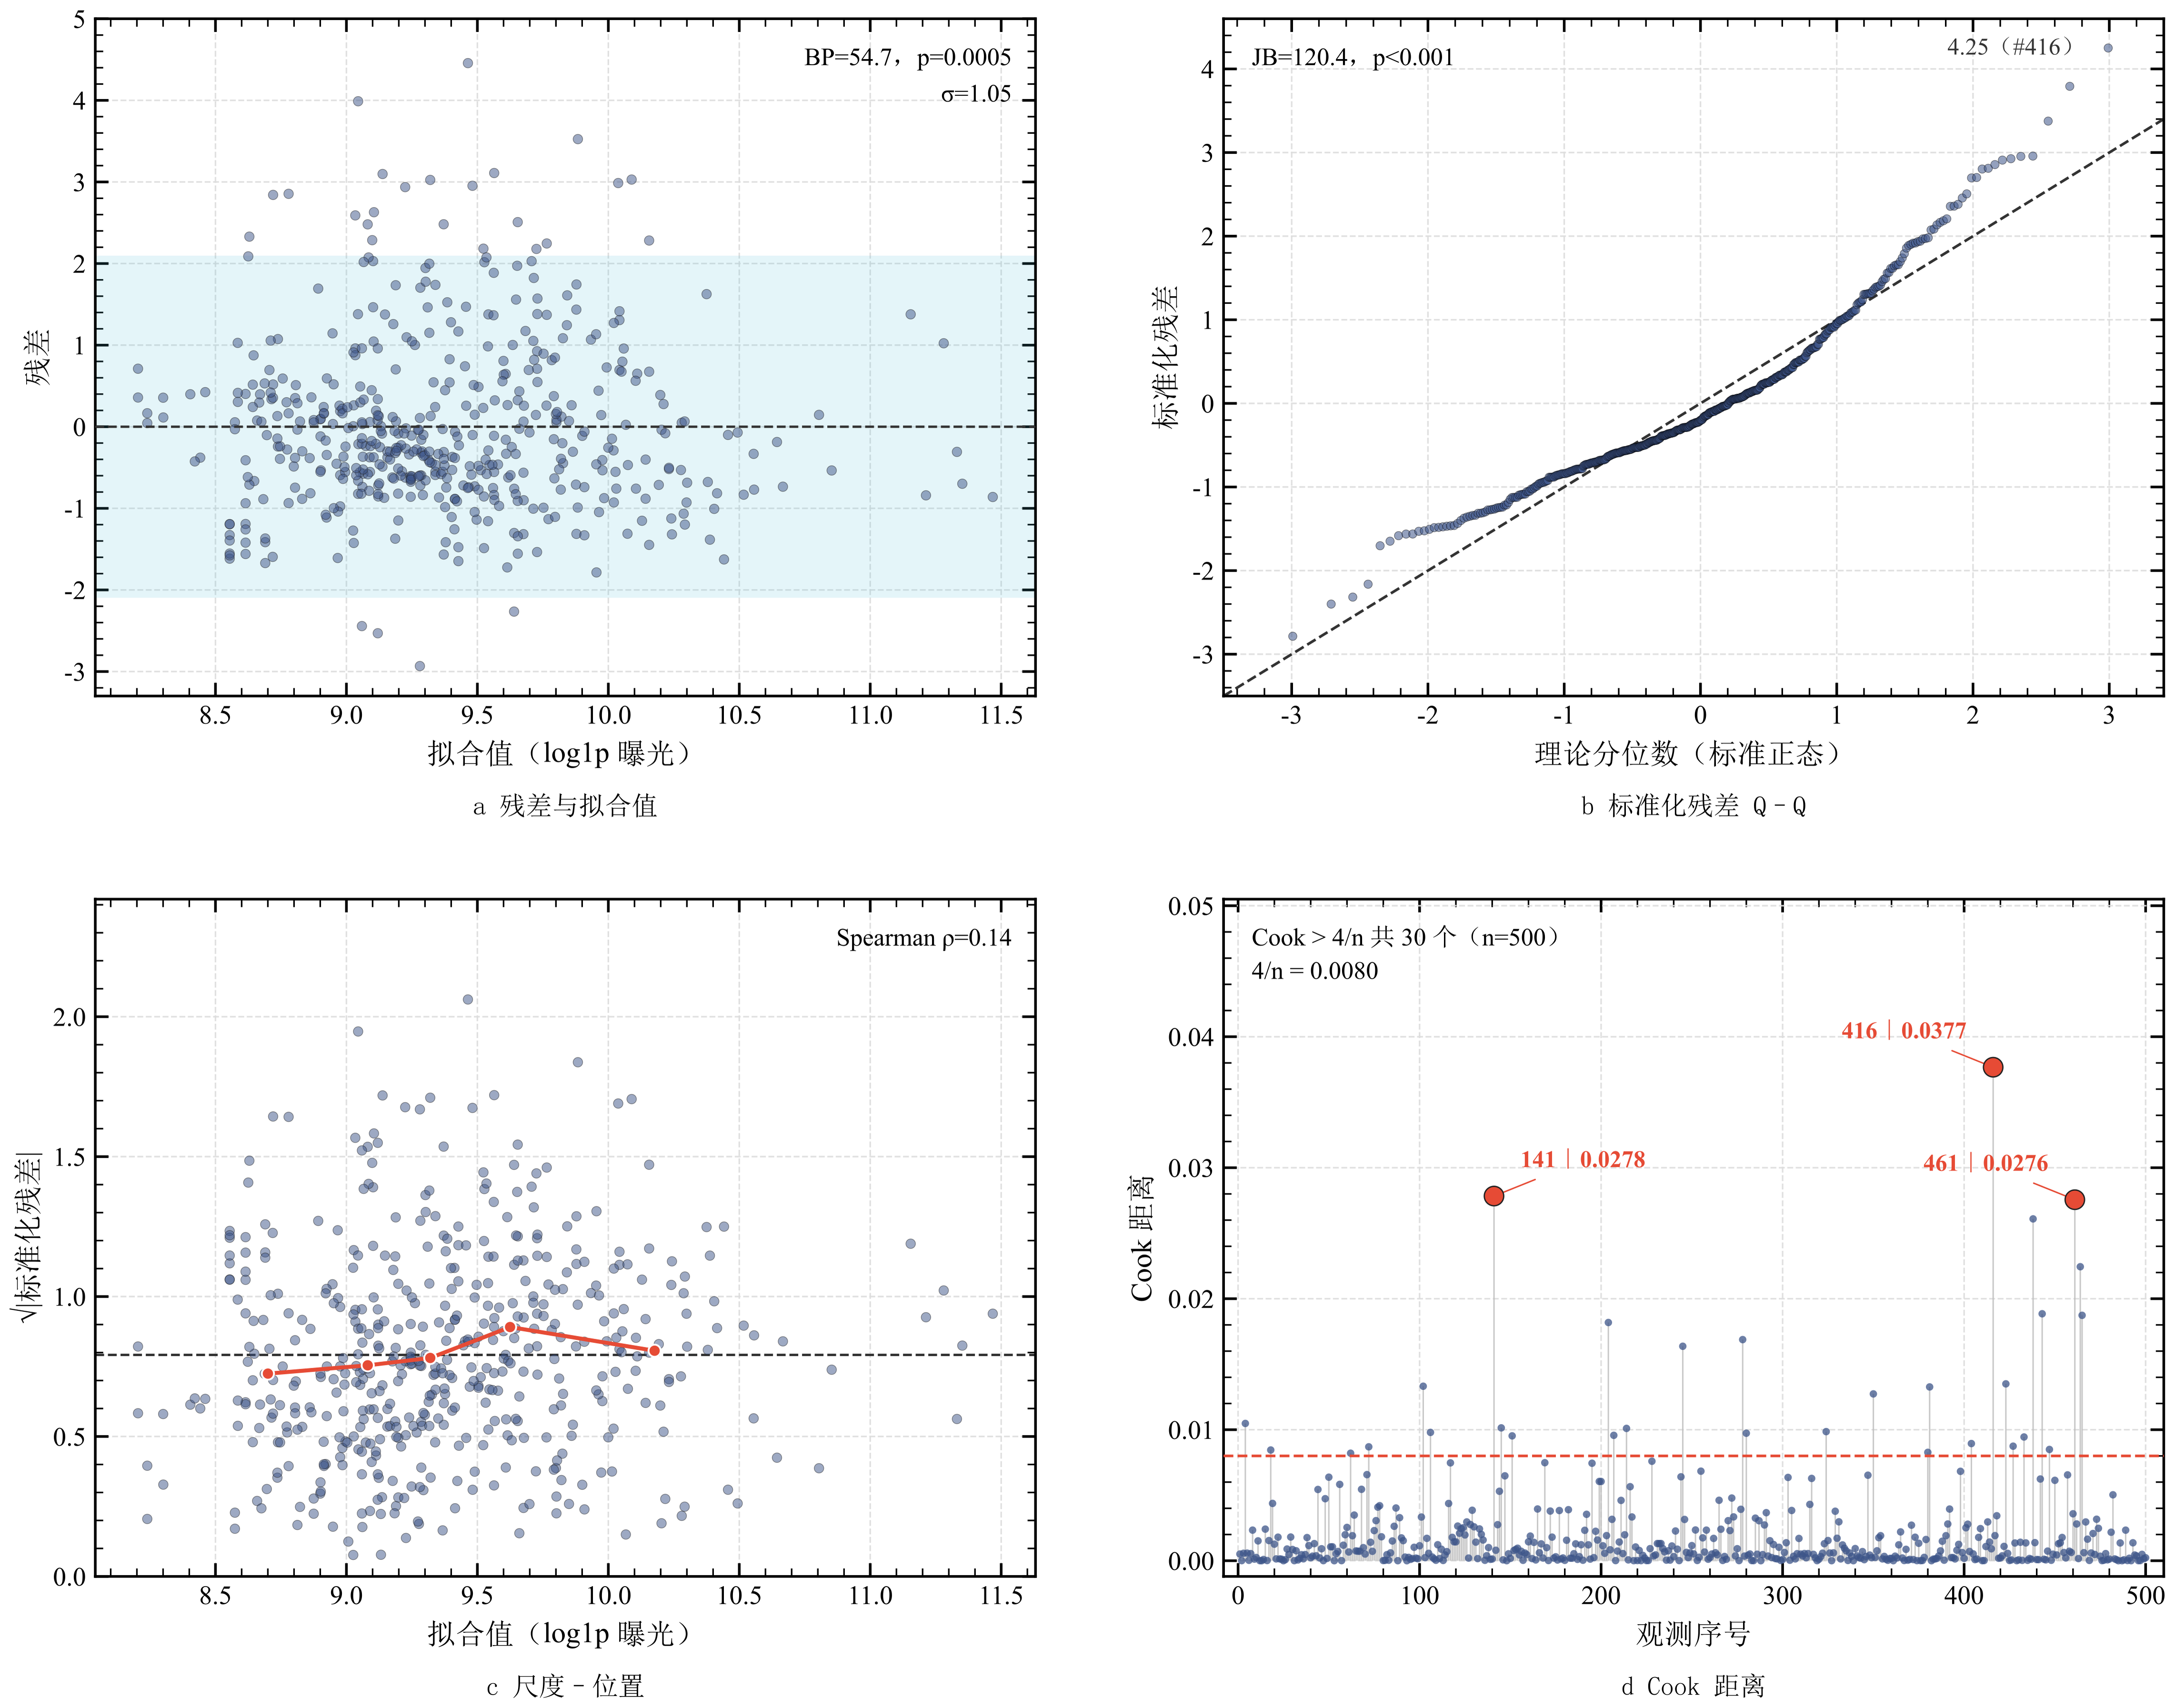
\includegraphics[width=0.68\textwidth]{../求解/问题三/结果/图8_残差诊断.png}
  \caption{最终模型残差诊断}
  \label{fig:q3_resid}
\end{figure}

图\ref{fig:q3_cv}对比样本内与交叉验证表现。左图中各模型的 CV $R^2$ 都低于样本内 $R^2$，M2 由 0.2068 降至 0.1010，降幅约一半，说明模型存在一定过拟合，但方向仍为正；M1 的降幅更大，M0 的 CV $R^2$ 为负。右图为 M2 的交叉验证预测与观测对照，点云沿 45 度线分布，但离散程度较大，CV $R^2$ 仅 0.101、RMSE 1.101、MAE 0.833，说明单条帖子的曝光量很难被完全预测，模型的价值在于识别平均效应而非精确点预测。

\begin{figure}[ht]
  \centering
  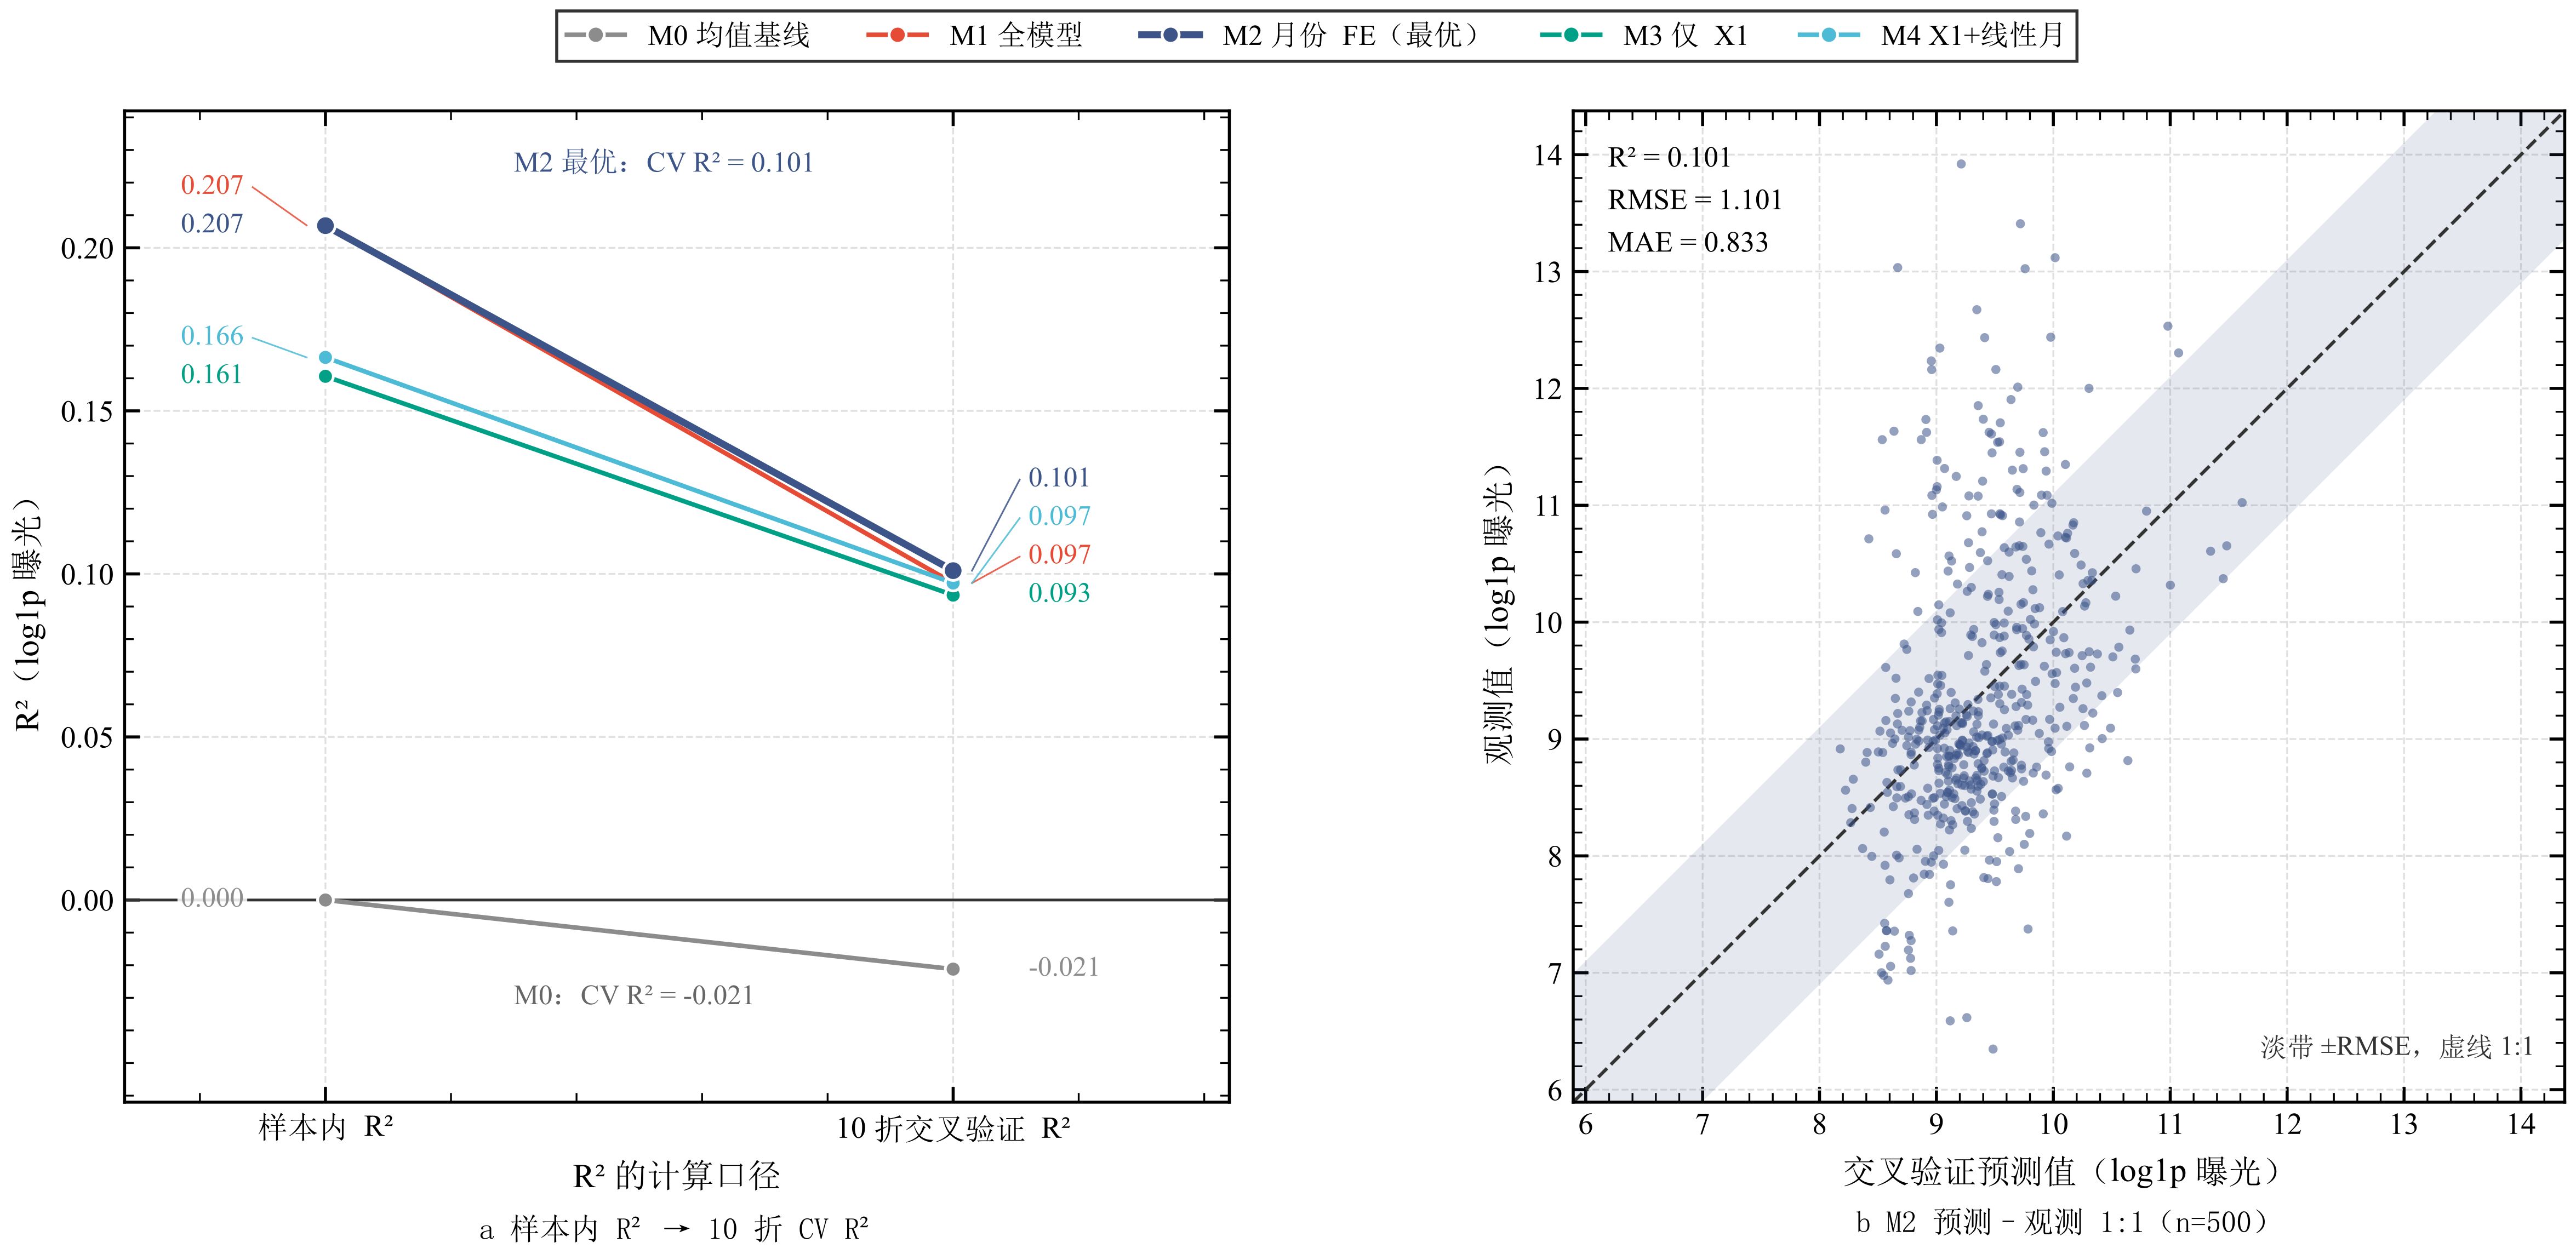
\includegraphics[width=0.72\textwidth]{../求解/问题三/结果/图9_预测能力验证.png}
  \caption{样本内与交叉验证预测能力}
  \label{fig:q3_cv}
\end{figure}

最后给出方差分解。表\ref{tab:q3_shapley}显示，帖子类型 X2 的 Shapley 贡献为 0.0767，占已解释方差的 37.1\%，是单一变量组中最大的；月份 X4 为 0.0579、占 28.0\%；付费 X7 为 0.0244、占 11.8\%；星期 X5 为 0.0236、占 11.4\%；内容主题 X3 为 0.0142、占 6.9\%；时段 X6 为 0.0055、占 2.6\%；粉丝规模 $\log X_1$ 仅为 0.0046、占 2.2\%。按类别合并，发帖决策合计解释 0.1445，占总方差的 14.45\%；账号规模与时间合计解释 0.0624，占 6.24\%；未解释部分为 0.7931，占 79.31\%。

\begin{longtable}{>{\centering\arraybackslash}p{0.26\textwidth}>{\centering\arraybackslash}p{0.12\textwidth}>{\centering\arraybackslash}p{0.14\textwidth}>{\centering\arraybackslash}p{0.14\textwidth}>{\centering\arraybackslash}p{0.18\textwidth}}
  \caption{Shapley 方差分解}
  \label{tab:q3_shapley} \\
  \toprule
  变量组 & 自由度 & Shapley $R^2$ & 占已解释方差 & 占总方差 \\
  \midrule
  \endfirsthead
  \caption{Shapley 方差分解（续）} \\
  \toprule
  变量组 & 自由度 & Shapley $R^2$ & 占已解释方差 & 占总方差 \\
  \midrule
  \endhead
  \bottomrule
  \endfoot
  发帖类型 X2 & 3 & 0.0767 & 37.1\% & 7.67\% \\
  内容主题 X3 & 2 & 0.0142 & 6.9\% & 1.42\% \\
  月份 X4 & 11 & 0.0579 & 28.0\% & 5.79\% \\
  星期 X5 & 6 & 0.0236 & 11.4\% & 2.36\% \\
  时段 X6 & 2 & 0.0055 & 2.6\% & 0.55\% \\
  付费 X7 & 1 & 0.0244 & 11.8\% & 2.44\% \\
  粉丝规模 $\log X_1$ & 1 & 0.0046 & 2.2\% & 0.46\% \\
  发帖决策合计 & 13 & 0.1445 & 69.8\% & 14.45\% \\
  规模与时间合计 & 12 & 0.0624 & 30.2\% & 6.24\% \\
  未解释方差 & — & 0.7931 & — & 79.31\% \\
\end{longtable}

图\ref{fig:q3_shapley}把上述分解可视化。左图按贡献从小到大排列七个变量组，决策类变量用深蓝、规模与时间类用红色区分；右图把总方差拆为发帖决策 14.45\%、规模与时间 6.24\% 与未解释 79.31\% 三段。发帖决策的贡献是规模与时间的两倍以上，说明可操控的内容与投放选择比账号自然增长更能解释帖子间的曝光差异；但两者合计仍不足总方差的四分之一，绝大多数变异来自未被观测到的推荐算法、受众匹配与传播随机性。

\begin{figure}[ht]
  \centering
  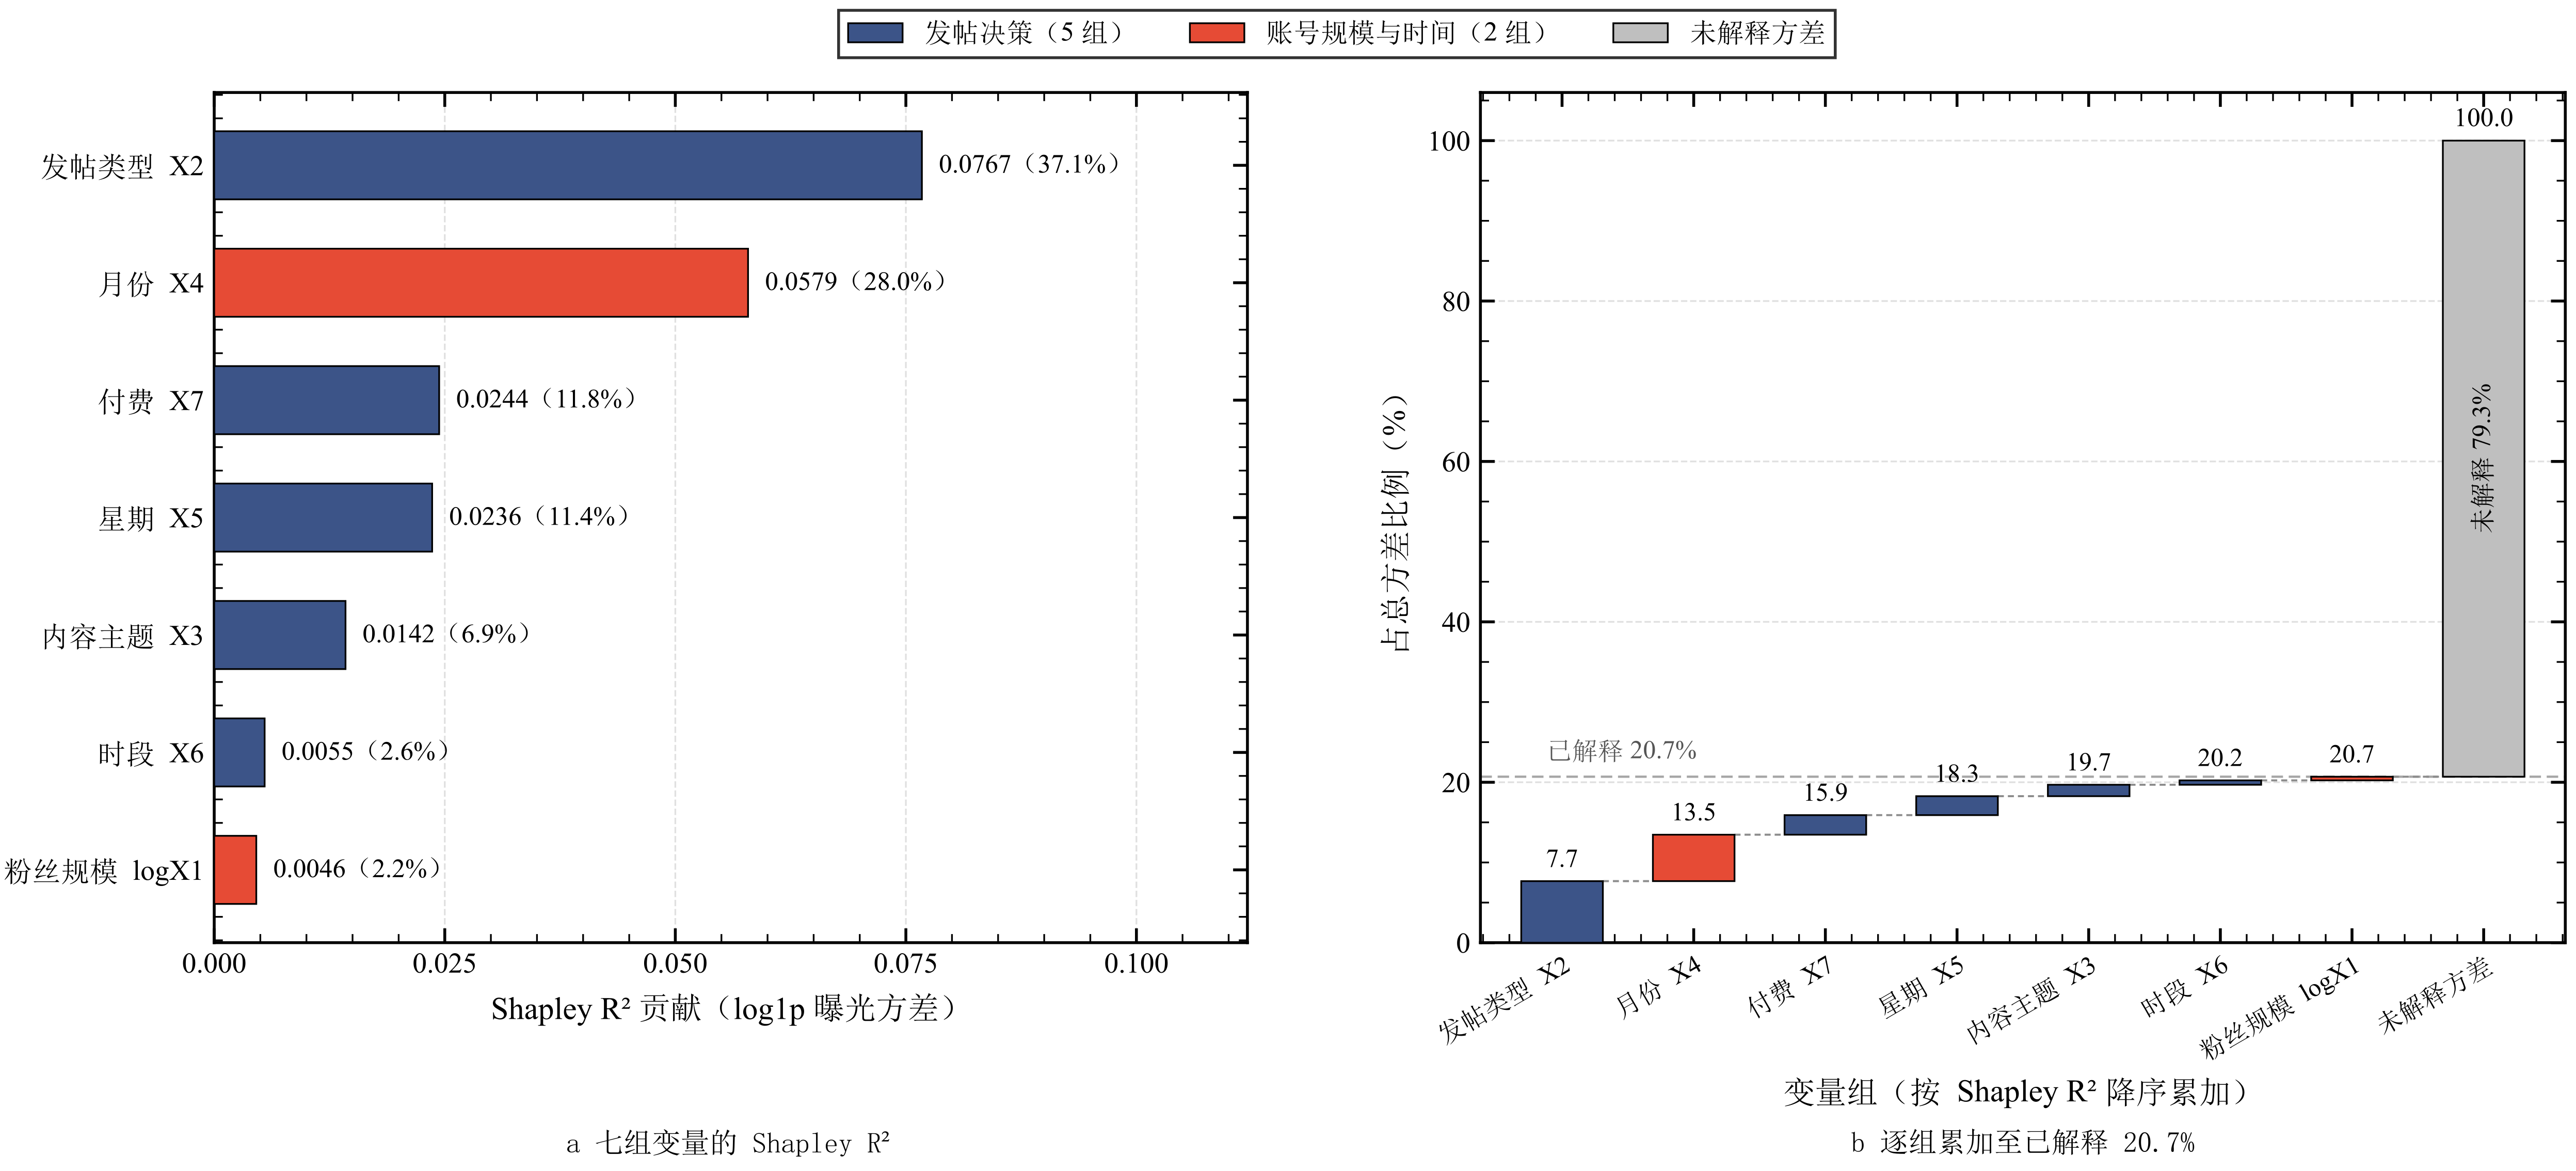
\includegraphics[width=0.75\textwidth]{../求解/问题三/结果/图10_方差贡献Shapley.png}
  \caption{变量组的 Shapley 方差贡献与总方差构成}
  \label{fig:q3_shapley}
\end{figure}

综合以上结果，M1 的粉丝规模系数在共线下不可识别，M2 以月份固定效应替代后共线消除、拟合几乎不变、交叉验证略优。最终模型在整体显著性与残差诊断上基本合格，样本外 $R^2$ 为 0.101，能够支撑平均效应测算，但不适合对单条帖子做精确点预测。发帖决策解释 14.45\% 的曝光方差，是后续效应测算的重点对象。
